\chapter{Filesystem Security}

It's all about the data! Whether hackers infiltrate a network and encrypt data for ransomware or whether data is stolen for its value (secrets, credit card numbers etc), there are an endless number of attacks against systems, often with the goal of getting to the data at the heart of an organization.

This chapter explores various security aspects surrounding the data that filesystems store. Encryption and key management are discussed in detail together with the standards that demand their deployment and govern their use. Some unusual topics like how to exploit previously allocated filesystem blocks to potentially located sensitive data will be described together with fixes that may or may not be applied depending on the filesystem and performance characteristics needed.

Two of the main Linux security subsystems, SELinux and AppArmor will be highlighted, specifically as both apply to filesystem access.

%Hackers hijack Linux devices using PRoot isolated filesystems
%
%https://www.bleepingcomputer.com/news/security/hackers-hijack-linux-devices-using-proot-isolated-filesystems/

%https://www.linuxtopia.org/online_books/linux_administrators_security_guide/06_Linux_File_System_and_File_Security.html

%https://www.secur.cc/how-to-secure-a-linux-file-system/

% Google "linux filesystem exploits"

\section{It Starts With File and Directory Permissions}

We've already discussed how the standard UNIX file permissions model is supposed to work. Let's discuss it's weaknesses and what can be done to alleviate these issues.

\textbf{find issues - setuid bit etc etc - NFS?}

\section{Encryption and Key Management}\label{encryption}

Our encrypting FUSE filesystem was a fun exercise and although file names and data are encrypted on disk, it is not a secure system. If someone got hold of the embedded encryption key, they have access to data. Most encryption systems use published encryption algorithms so if you have the key and know the encryption algorithm, you will be able to decrypt the data.

Furthermore, in our example of encryption in FUSE, we used a \textit{hard-coded encryption key} which is not at all secure. One key for all mounted filesystems and everywhere? Traditional laptop encryption used a password scheme where the encryption key is derived from the password. We could enhance the FUSE solution to do something similar but most enterprise encryption solutions require operating in a hands-off mode.

Figure \ref{fig:key-mgt} shows the components that may be used in an enterprise key management solution for providing filesystem encryption for Linux servers.

\begin{figure}
	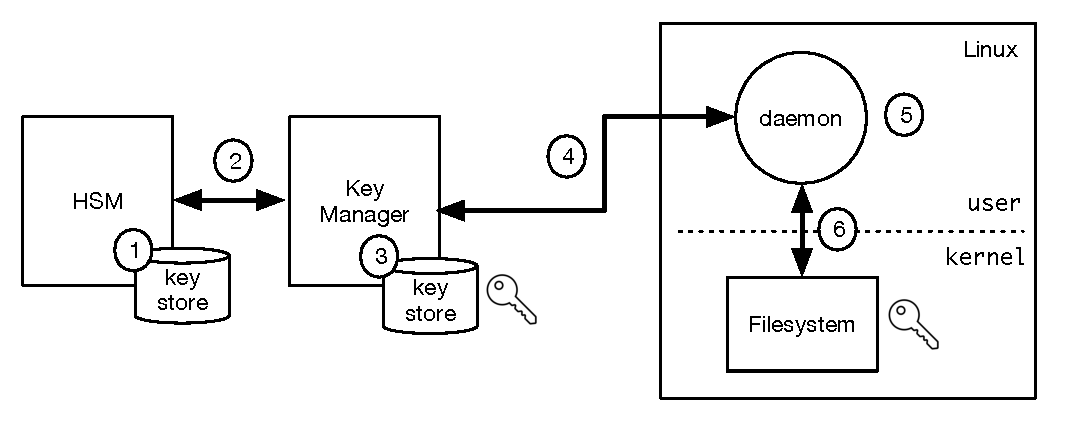
\includegraphics[scale=0.6]{figures/key-mgt.pdf}
	\centering
	\caption{Components in an enterprise encryption solution}
	\label{fig:key-mgt}
\end{figure}

\noindent
Here are the paths followed for key management:

\begin{enumerate}
	\item An HSM may be used to generate the key(s) used to encrypt filesystem data. These keys are called DEKs (Data
		Encryption Keys). They may be generate on demand from the key manager (KM). Alternatively, the KM may 
		generate its own keys using a local random source (either software or hardware). 
	\item Whether a DEK or a wrapping key, the key manager will request such keys from the HSM.
	\item A wrapping key may be used to unwrap (decrypt) one or more keys that are used to encrypt a key store on the KM.
	\item DEKs are send to the encryption agent over TLS and typically with an additional layer of \textit{wrapping} (extra
		layer of encryption). This will usually be in response to an event such as mounting a filesystem.
	\item The DEK is delivered to a filesystem module. There is likely additional wrapping between the daemon and
		the filesystem module.
	\item The DEK will be held in memory and used to encrypt / decrypt data as it passes to / from disk. The key
		may be protected in memory when not in use but will be decrypted (in the clear) in memory when in use.
\end{enumerate}

\noindent
Many commercially available, enterprise encryption solutions will have a KM deployed but many will not use an HSM. There is certainly a cost factor involved but the extra level of integration is typically only done for the most secure environments.

\subsection{Password-based Encryption}

UNIX passwords used to reside in the file \cf{/etc/passwd} which each line looked like the following:

\begin{lstlisting}
root:Ep6mckrOLChF:0:1:System Operator:/:/bin/ksh 
daemon:*:1:1::/tmp: 
uucp:POE9oN9NE:4:4::/var/spool/uucppublic:/usr/lib/uucp/uucico 
dennis:eH5/.jN7B3mdc:181:100:Dennis Ritchie:/u/dennis:/bin/ksh 
ken:fwkf5j1Tif4o.:182:100:Ken Thompson:/u/ken:/bin/csh
\end{lstlisting}

\noindent
The odd thing was that this file was readable by everyone. I had great fun in the late 1980s by running the \cf{crack} program on this file and showing our system administrator what the root password was. Each password was hashed using \cf{crypt(3)} so all the \cf{crack} program needed to do was brute force the password by trying one guess after another.

\textbf{I can't find crack anywhere. sshcrack perhaps?}. Nowadays john the ripper does something similar
 
The 1979 paper \textit{Password Security: A Case History} by Robert Morris and Ken Thompson is a very interesting read as they discuss issues with the original password scheme.
 
 \begin{table}[h]
\begin{tabular}{lcl}
\parbox[r]{0.5in}{
\includegraphics[scale=0.15]{figures/url.png}} & \parbox[l]{0.5in}{URL \arabic{urls} --} & \parbox[l]{3in}{\cf{https://tinyurl.com/2je3dd9e}}
\end{tabular}
\end{table}
\stepcounter{urls}
% https://rist.tech.cornell.edu/6431papers/MorrisThompson1979.pdf
 
\noindent
As a side note, I was super happy to find out a few years ago that Ken Thompson is still going strong and was one of the creators of Golang, a new language developed by Thompson together with Rob Pike and Robert Griesemer, all of whom now work for and Google.

There was a move away from using \cf{/etc/passwd} to store passwords in the mid 1980s but took time to roll out and be adopted by other vendors and of course Linux.

\subsection{Encryption Algorithms and Key Sizes}

There are many different encryption algorithms available today but by far, the most commonly used encryption algorithm used for file and disk encryption is AES, the \textit{Advanced Encryption Standard} with typical key sizes of 128 and 256 bytes. Most encryption systems have 256-byte keys as default. The next sessions discusses Intel hardware support for AES for key sizes and 128, 192 and 256 bits.

\textbf{CBC, XTS, ESSIV etc ...}

\subsection{Hardware Acceleration of AES}

Crypto is time-consuming especially when using software algorithms. When standing in front of customers, the question of performance would always come up and we would always talk around it and show the best numbers we had. Of course, if a databases has an extensive cache, the overhead is less depending on the benchmark. But software-based encryption generally has a high overhead and performance can be dreadful.

There have been many hardware based solutions over the years typically some form of card that is plugged into the motherboard. HSMs can be used to offload some crypto functions but not for file I/O operations. The trip over the write would add an unbearable overhead. 

AES is by far the most popular algorithm used for symmetric encryption. Intel introduced hardware support for AES with the introduction of AES-NI (Advanced Encryption Standard New Instructions) in 2008. It is an extension to the x86 instruction set architecture and has been enhanced many times over successive generations of Intel processors. Furthermore, the instructions are supported by the guest operating systems of all major hypervisor vendors. Support for AES-NI was added to the Linux kernel many years ago and can be used by any component inside the kernel.

For implementing encryption at the filesystem level, the performance gains are huge. How much gain is obtained is very depending on the type of I/O that applications are performing (as with all performance tests) but have reduced the encryption overhead to \textit{noise} rather than having a significant impact when using only software-based encryption.

\subsection{Access Controls}

UNIX/Linux has provided permissions at the file-level since UNIX first made its appearing in the late 1960s. While the user/group/other level of permissions is fine for general usage, it's possible for privileged users to be able to gain access to data for general users.

Encryption and enterprise key management, which will be covered in the next section, goes a long way to protect sensitive data but concerns still exist around ensuring only the right users and applications are accessing the decrypted data. This is particularly problematic on Linux since the root administrator can access non-root owned data. Security frameworks such as SELinux which will be described in section \ref{selinux} can help with preventing root from accessing data but the implementation is quite cumbersome. There are commercial products on the market such as Thales CTE (Ciphertrust Transparent Encryption), the old Vormetric products I worked on, which provide additional access controls that have capabilities such as:

\begin{itemize}
	\item Prevent root users from accessing specified paths under any circumstance.
	\item Zero-downtime encryption (for encrypting data that already exists).
	\item Only allow specific binaries to access data and ensure that these binaries haven't been tampered with through
		use of checksums.
\end{itemize}

\noindent
The encryption suite comes with FIPS 140-2 validated key management and highly-secure HSMs (Hardware Security Modules).

\subsection{EKM -- Enterprise Key Management and FIPS}

When selling key management into federal government and highly-regulated industries such as banking, obtaining FIPS 140-2/3 certification is a must.

It is generally a requirement for key managers to be at least FIPS 140-2 Level 1 certified since many of the key managers available today are run as virtual machines. Level 1 is generally the highest level of certification for a software component. The component that completes FIPS certification is called the \textit{cryptographic module}. This could be a single program or could be the whole operating system shipped to customers in different formats but could be a virtual appliance.

With level 1, at least one \textit{approved} cryptographic algorithm must be validated. This is achieved by running \textit{Known Answer Tests} (KAT) against the algorithm where the inputs and outputs are known ahead of testing. KAT are used to validate the algorithm in order to obtain a valid certificate for the algorithm and also performed during system initialization to make sure nothing has been tampered with and the algorithm still performs as expected. There is also a lot of scrutiny around which random number generator is used since that is the seed used for key generation. There are also other aspects of level 1 including taking checksums of components in the module and validating the components against the checksums on system initialization.

Above level 1, physical hardware must be used since level 2 above require tamper detection through hardware mechanisms and if an attempt is made to break into a physical FIPS appliance, keys will be shredded rendering the appliance useless.

FIPS 140-2 only validates the module once development is completed and yes, changes to reach certification, may result in a new version of the product being produced. At the time of writing, FIPS 140-2 is coming to an end and being replaced by FIPS 140-3 requires evaluation of  security requirements during all stages of the cryptographic module creation including design, implementation, and final operational deployment.

All modules certified by NIST have a \textit{Security Policy} that describes the module including algorithms certificates and all security policies can be found on the NIST website. I've gone through this process several times. An example of one of my security policies can be located on the NIST website here:

\begin{table}[h]
\begin{tabular}{lcl}
\parbox[r]{0.5in}{
\includegraphics[scale=0.15]{figures/url.png}} & \parbox[l]{0.1in}{\arabic{urls}} & \parbox[l]{3in}{\cf{https://tinyurl.com/3vzee5xe}}
\end{tabular}
\end{table}
\stepcounter{urls}
% https://csrc.nist.gov/projects/cryptographic-module-validation-program/certificate/2524

\noindent
You can see the algorithms validated and a link to the security policy.

\subsection{Common Criteria}

Most encryption and key management vendors cringe when the topic of Common Criteria is brought up by customers. FIPS 140-2 can be a costly and time-consuming exercise but nothing when it comes to the Common Criteria (CC) standard.

Where the FIPS component being evaluated is called the cryptographic module, in CC, it's the \textit{Target of Evaluation} (TOE). CC comprises several different \textit{Protection Profiles} (PP) and it's often not a trivial task to determine which CC a solution will fit under.

It will be left as an exercise to the reader to discover more about CC although I suspect most will only do so if required.

\subsection{HSMs -- Hardware Security Modules}

Providing the ultimate secure storage of secrets (encryption keys, certificates and so on), HSMs have been around for many years and have higher-levels of FIPS compliance since they will generally come in a highly secured physical appliance that is tamper proof. 

There are also specialized HSMs for different industries including payment HSMs which provide high levels of protection for cryptographic keys and customer PINs used during the issuance of magnetic stripe and EMV (Europay, Mastercard, and Visa) chip cards (and their mobile application equivalents) and the subsequent processing of credit and debit card payment transactions.

The functions of an HSM are:

\begin{itemize}
	\item Creation of crypto keys.
	\item Secure storage for crypto keys. Note that not all crypto keys are stored in the HSM but generally
		speaking, the most sensitive keys such as \textit{master keys} and \textit{wrapping keys} are
		typically stored in an HSM. 
	\item Key management functions including digital signature functions, offloading application servers 
		for complete asymmetric and symmetric cryptography.
	\item Manage transparent data encryption keys for databases and keys for storage devices such 
		as disk or tape.
\end{itemize}

\noindent
In the latter case, an HSM may be used to create and manage database keys but for filesystems and disks, a
key manager will typically be used since it generally has more context about the keys. In this keys, a higher-level
key that comes from the HSM may be used for the key store inside a key manager. 

HSMs are typically hardware appliances that are tamper proof including tamper detection and shredding of keys of seals are broken, wires tripped etc. One way of doing this is to use a physical HSM card inside the box that is wired to the chassis. If the chassis is tampered with (an attempt to open it), the wire will be pulled and keys will be shredded. 

They also have specialized hardware for key generation, crypto algorithms etc. But even with high-performant crypto acceleration, HSMs are not used for inline encryption of data through filesystems, the disk layer or for databases. It would be too much of a hit on performance to ship data back and forth across the wire between say a Linux server and an HSM. Instead, HSMs are often used in conjunction with a key manager (KM) where the KM may hold encrypted keys a filesystem might use but these keys are wrapped (encrypted themselves) with a key that is generated in the HSM and stored in the HSM.

\subsection{Protecting Keys Over the Wire}

For step 4 in figure \ref{fig:key-mgt}, an encryption key will come out of secure storage and be transported to the server where it will be used to encrypt/decrypt files and devices. TLS (Transport Layer Security) which was build on the now-deprecated SSL (Secure Sockets Layer) is used as a base layer of security by providing encryption of data over the wire. Various standards including Common Criteria will dictate the minimum version of TLS to use to avoid known vulnerabilities in earlier versions. 

But TLS is not enough by itself and is frowned up in security circles if that is the only method used to transport encryption keys. Some standards provide secure key exchange protocols and some encryption vendors also go beyond such standards with some rather elaborate schemes. In all cases asymmetric encryption is used to assist with the key exchange. 

The Diffie–Hellman key exchange protocol is one such method of providing secure exchange of keys between two parties. If you like mathematics, you are welcome to read about the algorithm on Wikipedia or view the NIST special publication here:

\begin{table}[h]
\begin{tabular}{lcl}
\parbox[r]{0.5in}{
\includegraphics[scale=0.15]{figures/url.png}} & \parbox[l]{0.1in}{\arabic{urls}} & \parbox[l]{3in}{\cf{https://tinyurl.com/2r93e6s5}}
\end{tabular}
\end{table}
\stepcounter{urls}
% https://nvlpubs.nist.gov/nistpubs/Legacy/SP/nistspecialpublication800-113.pdf

\subsection{Protecting Encryption Keys in Memory}

The previous sections have covered how keys can be securely generated, transported and stored \textit{at rest} (on disk storage for example) with hardware support and standardized protocols to ensure their safety. But with all of this, a key needs to be present when encryption/decryption takes place and will therefore be present in memory (in the clear). Some encryption products provided additional layers of security by unwrapping (decrypting) keys in memory only when needed and then wrapping (encrypting) them once the crypto operation has finished. But there is still a window when the keys are in clear-text and vulnerable to attack.

I recall many years ago when we demonstrated issues with encryption inside a VM to VMware and showed that, when we took a snapshot of the VM, we pulled the key out of the snapshot file. The issue is still there today.

This has been a major source of frustration for me for the last 15 years. There have been so many advances in memory protection by hardware vendors such as Intel but software support has been sorely lacking. And more specifically, we have been living in a virtualized world for many years but the hypervisor vendors have been slow to adopt some of these technologies. Furthermore, the hardware vendors have been designing in a vacuum with little consideration as to how such features will work through the hypervisor. Take VM live migration as an example. If CPUs are different XXX

Looking at some of the available technologies that can help with memory protection:

\begin{itemize}
	\item \textbf{Intel SGX} --- Intel Software Guard Extensions (SGX) allow applications to have protected private regions of 
		memory, called enclaves. Enclaves are areas of memory that are encrypted which prevent them from being
		read or examined by other programs. While promising, early versions of SGX had very limited space for enclaves
		and the technology only applies to user-level applications so it can't be deployed for filesystem or disk-level
		encryption.
	\item \textbf{Intel Total Memory Encryption (TME)} --- this provides encryption of memory which protects against physical 
		attacks to exfiltrate data. The CPU and RAM modules communicate over a bus on the motherboard, it's possible to 
		tap into this data bus allowing an attacker to read the contents of memory.
	\item \textbf{AMD Secure Encrypted Virtualization (SEV)} --- Like Intel TME, SEV provides encryption of all of the 
		memory of a virtual machine (VM) using a key per VM.
\end{itemize}

\noindent
While such technologies don't directly help with encryption of filesystem data, their main use is in protection of memory
where encryption keys are held. With some encryption technologies, keys themselves are wrapped (encrypted) in memory and only decrypted when in use but that still leaves a window when the key is visible.

\subsection{NIST Standards}

The United States National Institute of Standards and Technology (NIST) has many standards for encryption and key management including a set of public facing documents call special publications. Each special publication that has been written to address and support the security and privacy needs of U.S. Federal Government information and information systems is prefixed with "SP 800". Just run a web search for "nist sp 800" and you should see the following website:

\begin{table}[h]
\begin{tabular}{lcl}
\parbox[r]{0.5in}{ 
\includegraphics[scale=0.15]{figures/url.png}} & \parbox[l]{0.1in}{\arabic{urls}} & \parbox[l]{3in}{\cf{https://csrc.nist.gov/publications/sp800}}
\end{tabular}
\end{table}
\stepcounter{urls}
% https://csrc.nist.gov/publications/sp800

\noindent
There are a lot of documents on this page. Some examples include:

\begin{itemize}
	\item SP 800-12 -- An Introduction to Information Security
	\item SP 800-133 -- Recommendation for Cryptographic Key Generation
	\item SP 800-131A -- Transitioning the Use of Cryptographic Algorithms and Key Lengths
\end{itemize}

\subsection{Keep it Simple --- Encrypt it Yourself}

If you wish to transport encrypted files to a friend, family member or colleague, there are many commercial solutions available which are well beyond the scope of this book but there are open-source tools that allow you to achieve this with the \cf{openssl(1SSL)} command being one of the top choices. For information on how to do this, I recommend the following article:

\begin{table}[h]
\begin{tabular}{lcl}
\parbox[r]{0.5in}{
\includegraphics[scale=0.15]{figures/url.png}} & \parbox[l]{0.1in}{\arabic{urls}} & \parbox[l]{3in}{\cf{https://tinyurl.com/3b9d3t3y}}
\end{tabular}
\end{table}
\stepcounter{urls}
% https://opensource.com/article/21/4/encryption-decryption-openssl

\noindent
As with most things encryption related, the mathematics is complicated but most of the engineers who implement encryption solutions rarely have to delve that deep. Most encryption algorithms have publicly available implementations and most languages and support for hardware-based encryption is available everywhere including OpenSSL and inside the Linux kernel. 

\section{Zero Blocks / Extents on Allocation or Free}

Data allocated to a file is in blocks or extents which are general multiples of the disk sector size. To remove a file, each of these blocks/extents must be removed from the filesystem inode and added back to the free list. Generally speaking these blocks are not zeroed which is a timely operation. This means that when such blocks are allocated to a new file, the old contents remain and are potentially visible by the new owner.

Generally speaking, most applications won't see this stale data. If you create a file and write a file as follows:

\begin{lstlisting}
int
main()
{
    char *buf = "hello world\n";
    int  fd = open("/mnt/foo", O_CREAT|O_WRONLY, 0700);

    write(fd, buf, strlen(buf));
}
\end{lstlisting}

\noindent
You will see a file of the size determined by the amount of data written (12 bytes):

\begin{lstlisting}
$ [*\bfseries ls -l foo*]
-rw------- 1 spate spate 12 Dec 22 16:55 foo
\end{lstlisting}

\noindent
If you try to read beyond the file, you will get an error XXX. Furthermore, the data in the block is zeroed by the kernel so you won't see old data. \textbf{What about mmap?????? - need to find where the kernel zeroes blocks}. 

But a problem can exist. To demonstrate this, I'll use the disk-based SPFS which does not zero blocks that have be deallocated and reused. I have a file with 200 lines of fake credit card names and numbers. 

\begin{lstlisting}
American Express, Scott Davis,  47289...2804, 03/2026, CID: 3379
American Express, Hailey Jones, 34357...6656, 03/2026, CID: 6275
American Express, Maria Miller, 34784...6300, 03/2026, CID: 1391
...
\end{lstlisting}

\noindent
and simply copy the file into an SPFS-mounted filesystem:

\begin{lstlisting}
# [*\bfseries mount -t spfs /dev/sda /mnt*]
# [*\bfseries cp ../test/credit-card-nos /mnt*]
# [*\bfseries umount /mnt*]
\end{lstlisting}

\noindent
Inside the SPFS \cf{fsdb} we can locate the file, the allocated blocks inside the file and the read the contents of each block:

\begin{lstlisting}
spfsdb > [*\bfseries i4*]
inode number 4
  i_mode     = 81a4
  i_nlink    = 1
  i_atime    = Wed Dec 21 18:06:19 2022
  i_mtime    = Wed Dec 21 18:06:19 2022
  i_ctime    = Wed Dec 21 18:06:19 2022
  i_uid      = 0
  i_gid      = 0
  i_size     = 13774
  i_blocks   = 7
  [*\bfseries i\_addr[ 0] = 131*]   i_addr[ 1] = 132   i_addr[ 2] = 133 
  i_addr[ 3] = 134   i_addr[ 4] = 135   i_addr[ 5] = 136 
  i_addr[ 6] = 137 
spfsdb > [*\bfseries b131*]
0000  416d 6572 6963 616e 2045 7870 7265 7373  American Express
0020  3437 3238 3339 3838 3837 3238 3034 2c20  47283988872804, 
0040  3739 0a41 6d65 7269 6361 6e20 4578 7072  79.American Expr
0060  732c 2033 3433 3537 3436 3936 3133 3536  s, 3435746961356
0080  3a20 3632 3735 0a41 6d65 7269 6361 6e20  : 6275.American 
00a0  696c 6c65 722c 2033 3437 3834 3831 3831  iller, 347848181
....
\end{lstlisting}

\noindent
This alone presents a security issue to many given that the root administrator can access sensitive data through the device interface. 

But let's get back to the example in hand. We're going to remove this file and create a new file with the following program:

\begin{lstlisting}
#include <stdio.h>
#include <fcntl.h>
#include <unistd.h>
#include <string.h>

int
main(int argc, char *argv[])
{
    char *buf = "hello world\n";
    int fd = open("/mnt/foo", O_CREAT|O_WRONLY, 0700);

    lseek(fd, 2030, SEEK_SET);
    write(fd, buf, strlen(buf));
}
\end{lstlisting}

\noindent
Let's give it a run and see what happens:

\begin{lstlisting}
# [*\bfseries mount -t spfs /dev/sda /mnt*]
# [*\bfseries rm /mnt/credit-card-nos *]
# [*\bfseries ./seeker*]
# [*\bfseries cat /mnt/foo *]
American Express, Scott Davis,  3472...72804, 03/2026, CID: 3379
American Express, Hailey Jones, 3435...35656, 03/2026, CID: 6275
American Express, Maria Miller, 3478...46300, 03/2026, CID: 1391
...
American Express, Bradley Henry, 3768...5450, 03/2026, CID: 5787
American Express, Frank Robinson[*\bfseries hello world*]
\end{lstlisting}

\noindent
Voila! There are some of the contents of the old file. Our "\cf{hello world}" string is there where we wrote it (highlighted in bold).

You would not see the same thing if we run the following:

\begin{lstlisting}
# [*\bfseries cp ../test/credit-card-nos /mnt*]
# [*\bfseries rm /mnt/credit-card-nos *]
# [*\bfseries echo hello > /mnt/foo*]
# [*\bfseries cat /mnt/foo*]
hello
\end{lstlisting}

\noindent
and looking at the allocated block using \cf{fsdb}:

\begin{lstlisting}
spfsdb > [*\bfseries b131*]
0000  6865 6c6c 6f0a 0000 0000 0000 0000 0000   hello...........
0020  0000 0000 0000 0000 0000 0000 0000 0000   ................
0040  0000 0000 0000 0000 0000 0000 0000 0000   ................
\end{lstlisting}

\noindent
\textbf{XXX---need to say why. Page allocated and zeroed}

\subsection{Fixing the Issue}

There are several ways to fix this issue or a fix may not be needed at all if there is no sensitive data in the filesystem. The first way is to zero a block every time it's allocated. If you look at \cf{sp\_block\_alloc()} it simply looks through the in-core SPFS superblock to see if a block is available. Here is the snippet of code with the check highlighted:

\begin{lstlisting}
    mutex_lock(&sbi->s_lock);
    for (i = 1 ; i < SP_MAXBLOCKS ; i++) {
       [*\bfseries  if (sbi->s\_block[i] == SP\_BLOCK\_FREE) {*]
            sbi->s_block[i] = SP_BLOCK_INUSE;
            sbi->s_nbfree--;
            mutex_unlock(&sbi->s_lock);
            return SP_FIRST_DATA_BLOCK + i;
        }
    }
\end{lstlisting}

\noindent
There is no need to go to disk at this point although the superblock will be marked dirty and flushed to disk at some point. If we wish to zeroize the block, we don't want to read it from disk so we should call getblk, zero the block and mark it as dirty so it will be flushed at some point. Hmm! Won't work with the page cache or there may be issues. Need to look into this.

{\bfseries Also show quick fix in SPFS by zeroing blocks when freed}

\subsection{A DIY Solution}

The \cf{wipe(1)} command is an interesting option. The manpage gives reasons as to why taking matters into your own hands may be a good solution, especially when decommissioning disk drives. It highlights issues with newer filesystems where data may temporarily be stored in the filesystem journal (something we'll be covering in Volume 2) and even if deletion, how it's possible to recover data that was previously erased. And they state that the best way to sanitize a storage medium is to subject it to temperatures exceeding 1500K. I doubt anyone has a BBQ that can go to those temperatures. And furthermore, I have to quote this from the manpage:

\begin{quote}
\textit{I strongly recommend to call wipe directly on the corresponding block device with the appropriate options. However THIS IS AN EXTREMELY DANGEROUS THING TO DO.  Be sure to be sober.}
\end{quote}

\noindent
There are several options available for the command and it repeatedly writes over the data:

\begin{quote}
\textit{... wipe repeatedly overwrites special patterns to the files to  be  destroyed,  using  the fsync()  call  and/or  the  O\_SYNC  bit to force disk access. In normal mode, 34 patterns are used (of which 8 are random)}
\end{quote}

\noindent
Here is the \cf{wipe(1)} running to overwrite the contents of the credit card file:

\begin{lstlisting}
$ [*\bfseries wipe /mnt/dir/credit-card-nos*]
Okay to WIPE 1 regular file ? (Yes/No) [*\bfseries Yes*]
Wiping /mnt/dir/credit-card-nos, pass 34 (34)   
Operation finished.                                                           
1 file wiped and 0 special files ignored in 0 directories, 
0 symlinks removed but not followed, 0 errors occurred.
\end{lstlisting}

\noindent
Running the SPFS \cf{fsdb} command the contents of what was the first block of the file are displayed. This and all other blocks now have random data throughout.

\begin{lstlisting}
spfsdb > [*\bfseries b131*]
0000  047f 5e0c fc36 96ab 049f e200 7727 708f   ..^..6......w'p.
0020  54aa aff9 c1c9 84b1 d6ac 9632 7e92 d01f   T..........2~...
0040  ac26 c946 b034 90d8 50ef ed21 87a6 6e78   .&.F.4..P..!..nx
\end{lstlisting}

\noindent
It's safe to say that at this point, the old data has ceased to be.

If I was that concerned about the security of data I would encrypt the filesystem or disk, add appropriate access controls and make sure I had a good key management strategy. I recall a conversation with a Wall Street CISO several years ago. His CTO was concerned about encryption overheard. The CSO responded by asking how much it would cost for CPUs with slightly greater performance to compensate. If you want to be secure, don't be cheap! Data Breaches are very costly.

We added a block zeroize capability to VxFS many years ago in response to customer requests. This still left the problem of regular file data being present at times in the intent log. We'll come back to this topic on Volume 2.

\section{Security is a Multi-Layered Approach}

I remember many years when I first heard my friend and former colleague Mike Fleck talking about the M\&M model of security. \textit{Hard on the outside and soft on the inside}. In other words, an organization builds an impenetrable shell to the organization's infrastructure, taking the view \textit{“No one gets in unless we let them”}. But once you're on (or allowed to be in), you generally have free rein throughout the organization’s infrastructure. This always reminds me of figure \ref{fig:mm}.

\begin{figure}
	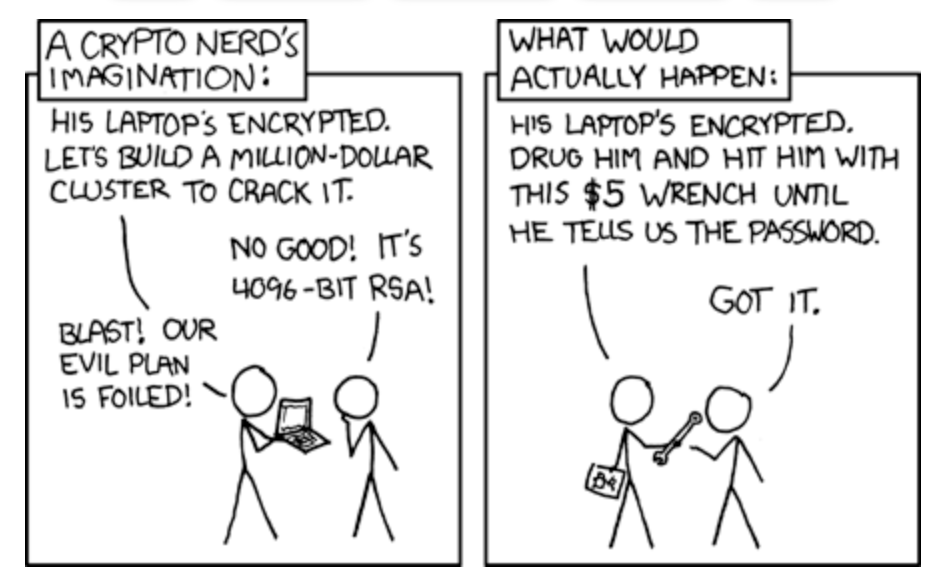
\includegraphics[scale=0.5]{figures/security.png}
	\centering
	\caption{How good is your security?}
	\label{fig:mm}
\end{figure}

Security vendors and customers are becoming more interested in the \cf{Zero Trust} model of security whereby they assume that they are operating in an environment where there is no traditional network edge. In other words, the M\&M model of security no longer applies. 

In the zero trust model, trust is never granted implicitly but must be continually evaluated. In other words "\textit{never trust, always verify}". Zero Trust was designed to protect modern environments and enable digital transformation by using strong authentication methods, leveraging network segmentation, preventing lateral movement, providing Layer 7 threat prevention, and simplifying granular, “least access” policies. 

The NIST Special Publication \textit{Zero Trust Architecture} (SP 800-207) is being adopted by some security vendors. It can be used as a base to understand the zero trust model and then see what the security vendors say in terms of their products. For many of them, they have multiple products which don't work well, or at all, together. A zero trust model should bring these products together to operate as a whole and give enterprise-level visibility and security.

\section{SELinux}\label{selinux}

Main benefits - su detection

out of the box still for RHEL as well as OpenShift.

lots of customers disable it straightaway 

Fedora Core 2 adopted SELinux back in 2004. It was then added to RHEL (Red Hat Enterprise Linux) in 2005 although it the aims were for maximum ease of use and therefore wasn't as restrictive as it could be. It was added to Ubuntu 8.04 (2008) and was in OpenSUSE 11.1 as a technical preview in \textbf{XXX?}

SE Linux and labeling files.

%https://access.redhat.com/documentation/en-us/red_hat_enterprise_linux/6/html/security-enhanced_linux/sect-security-enhanced_linux-working_with_selinux-selinux_contexts_labeling_files

\section{AppArmor}

TBD

\section{SELinux vs AppArmor}

TBD

% https://phoenixnap.com/kb/apparmor-vs-selinux - looks good

% https://www.redhat.com/sysadmin/apparmor-selinux-isolation - text below - modified

In general, SELinux is a more complex technology than AppArmor in that it controls more operations and \textit{separates containers by default???}. It's not possible to get this level of control using AppArmor due to the lack of MCS. In addition, not having MLS means that AppArmor cannot be used in highly secure environments. <- rewrite and understand.

from wikipedia

\begin{quote}
SELinux represents one of several possible approaches to the problem of restricting the actions that installed software can take. Another popular alternative is called AppArmor and is available on SUSE Linux Enterprise Server (SLES), openSUSE, and Debian-based platforms. AppArmor was developed as a component to the now-defunct Immunix Linux platform. Because AppArmor and SELinux differ radically from one another, they form distinct alternatives for software control. Whereas SELinux re-invents certain concepts to provide access to a more expressive set of policy choices, AppArmor was designed to be simple by extending the same administrative semantics used for DAC up to the mandatory access control level.

There are several key differences:

One important difference is that AppArmor identifies file system objects by path name instead of inode. This means that, for example, a file that is inaccessible may become accessible under AppArmor when a hard link is created to it, while SELinux would deny access through the newly created hard link.

As a result, AppArmor can be said not to be a type enforcement system, as files are not assigned a type; instead, they are merely referenced in a configuration file.

SELinux and AppArmor also differ significantly in how they are administered and how they integrate into the system.[34]
Since it endeavors to recreate traditional DAC controls with MAC-level enforcement, AppArmor's set of operations is also considerably smaller than those available under most SELinux implementations. For example, AppArmor's set of operations consist of: read, write, append, execute, lock, and link.[35] Most SELinux implementations will support numbers of operations orders of magnitude more than that. For example, SELinux will usually support those same permissions, but also includes controls for mknod, binding to network sockets, implicit use of POSIX capabilities, loading and unloading kernel modules, various means of accessing shared memory, etc.

There are no controls in AppArmor for categorically bounding POSIX capabilities. Since the current implementation of capabilities contains no notion of a subject for the operation (only the actor and the operation) it is usually the job of the MAC layer to prevent privileged operations on files outside the actor's enforced realm of control (i.e. "Sandbox"). AppArmor can prevent its own policy from being altered, and prevent file systems from being mounted/unmounted, but does nothing to prevent users from stepping outside their approved realms of control.

For example, it may be deemed beneficial for help desk employees to change ownership or permissions on certain files even if they don't own them (for example, on a departmental file share). The administrator does not want to give the user(s) root access on the box so they give them CAP\_FOWNER or CAP\_DAC\_OVERRIDE. Under SELinux the administrator (or platform vendor) can configure SELinux to deny all capabilities to otherwise unconfined users, then create confined domains for the employee to be able to transition into after logging in, one that can exercise those capabilities, but only upon files of the appropriate type.[citation needed]
There is no notion of multilevel security with AppArmor, thus there is no hard BLP or Biba enforcement available.[citation needed].
AppArmor configuration is done using solely regular flat files. SELinux (by default in most implementations) uses a combination of flat files (used by administrators and developers to write human readable policy before it's compiled) and extended attributes.
SELinux supports the concept of a "remote policy server" (configurable via /etc/selinux/semanage.conf) as an alternative source for policy configuration. Central management of AppArmor is usually complicated considerably since administrators must decide between configuration deployment tools being run as root (to allow policy updates) or configured manually on each server.
\end{quote}

\section{Security Standards}

There are many standards out that that deal with security. I suspect that readers will have heard of some but certainly not all. For example, we all hear about HIPPA (the \textit{Health Insurance Portability and Accountability Act}) as we come across it each time we visit the doctor, dentist or optometrist. If you deal with government organizations you'll certainly have heard of FIPS. Of course GDPR (General Data Protection Regulation) and its California equivalent CCPA (California Consumer Protection Act) together with huge fines that organizations are having to pay are often in the news

In the banking space, the Payment Card Industry PCI DSS (\textit{Data Security Standard}) have a set of guidelines that must be followed by vendors who are storing credit cards. You may have seen the term PCI 2.0.

At the operating system level, there are a lot of different standards. On the Red Hat website, this is what they list that they support just for the government space including FIPS and CC which were discussed earlier.

\begin{enumerate}
	\item COMMON CRITERIA
	\item FIPS 140-2 and FIPS 140-3
	\item Secure Technical Implementation Guidelines (STIG)
	\item Criminal Justice Information Services (CJIS)
	\item US Government Configuration Baseline (USGCB)
	\item USGv6-r1 TESTED PRODUCT LIST
	\item USGv6 TESTED PRODUCT LIST
	\item SECTION 508
	\item US ARMY CERTIFICATE OF NETWORTHINESS
	\item FISMA
	\item FedRAMP
	\item NISPOM CHAPTER 8
	\item HIPAA Overview
\end{enumerate}

\noindent
Not all are filesystem-related but many many have some implications on filesystem activity. Most people working on Linux, including the kernel may not come across many of these standards. It largely depends on the field in which you work. For engineers working on products in the security space, many will be familiar. Encryption and key management plays a re large part in several of these standards, some times as recommendations (HIPPA) and sometimes as mandates (PCI).

\section{Secure Programming}

% https://snyk.io/learn/secure-coding-practices/

Need to think about whether to include this or not.

\section{Conclusion}

Security is a large topic and anyone who has been to the RSA show in San Francisco held in winter each year will know how big a field this is and how much it has grown. While it is not always imperative for engineers to be aware of what standards are out there, it's important to have some level of awareness of the issues and what can be done to protect against vulnerabilities or attackers. Hopefully this chapter provided insight into the most important topics.

